% !TeX spellcheck = en_GB
For the simplest case of $N = 2$, we generate data sets of size $N_{\mathrm{data}} = 20000$ for $\rho_0 = \ket{0} \bra{0}, \ket{+} \bra{+}$ and random pure states.
The Drive qubits are sampled randomly from the Haar measure \cite{Mezzadri}.
We train each data set on a fully-connected feedforward ANN with a single hidden layer with 10 neurons.
The efficiency of the models is presented in Table \ref{n2efftable}.
For $N = 2$, starting in an eigenstate of the Drive Hamiltonian $H_{DS}$ gives the highest model efficiency, as the optimal Transducer policy is trivial to learn and implement (see appendix \ref{n2_opt_pol}).

For random initial states the efficiency is close to zero.
This is to be expected, as without knowledge of the system state $\rho_0$ the optimal Transducer policy cannot be determined.\footnote{The deviation from zero is a relic of the way the test data is shuffled. For $N_{\mathrm{data}} \to \infty$ it would disappear.}
We therefore train the same network with the random initial state as additional inputs using the same embedding as the Drive sequence.
This increases the test data efficiency, but is still far below the efficiency for $\rho_0 = \ket{+} \bra{+}$.


\begin{table}[h]
	\centering
	\begin{tabular}{ c | c }
		$\rho_0$ & $\eta_{test} \ [\%]$ \\
		\hline
		$\ket{0} \bra{0}$ & 72.7 \\
		$\ket{+} \bra{+}$ & 100.0 \\
		Random & 0.5 \\
		Random, $\rho_0$ as input & 43.0 \\
	\end{tabular}
	\caption{Efficiencies $\eta$ on the test data for models with a single hidden layer with 10 neurons trained on Drive protocols with $N = 2$ and differing initial states $\rho_0$.}
	\label{n2efftable}
\end{table}


%\begin{figure}
%	\centering
%	\begin{subfigure}{0.4\textwidth}
%		\centering
%		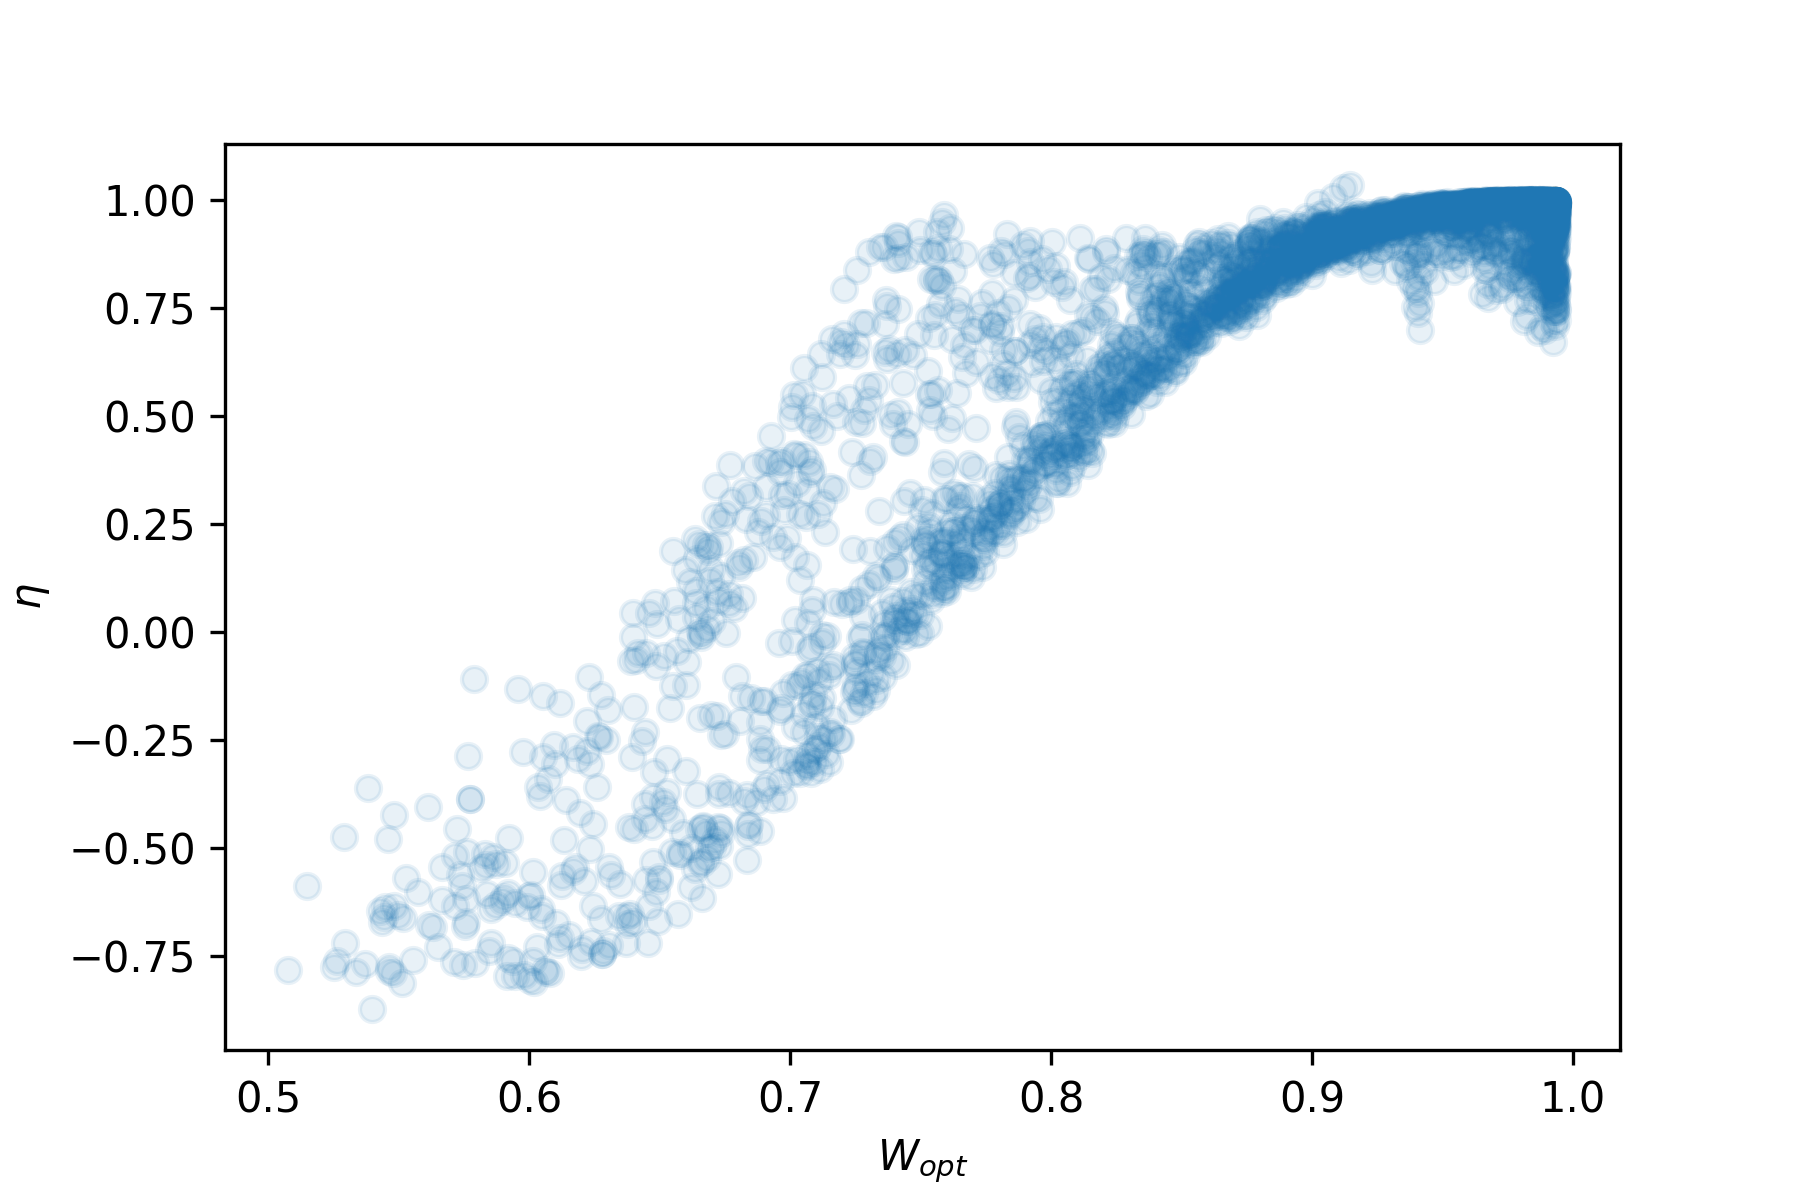
\includegraphics[width=\textwidth]{img/work_dist_n2_0}
%		\caption{$\rho_0 = \ket{0}\bra{0}$}
%		\label{}
%	\end{subfigure}
%	\begin{subfigure}{0.4\textwidth}
%		\centering
%		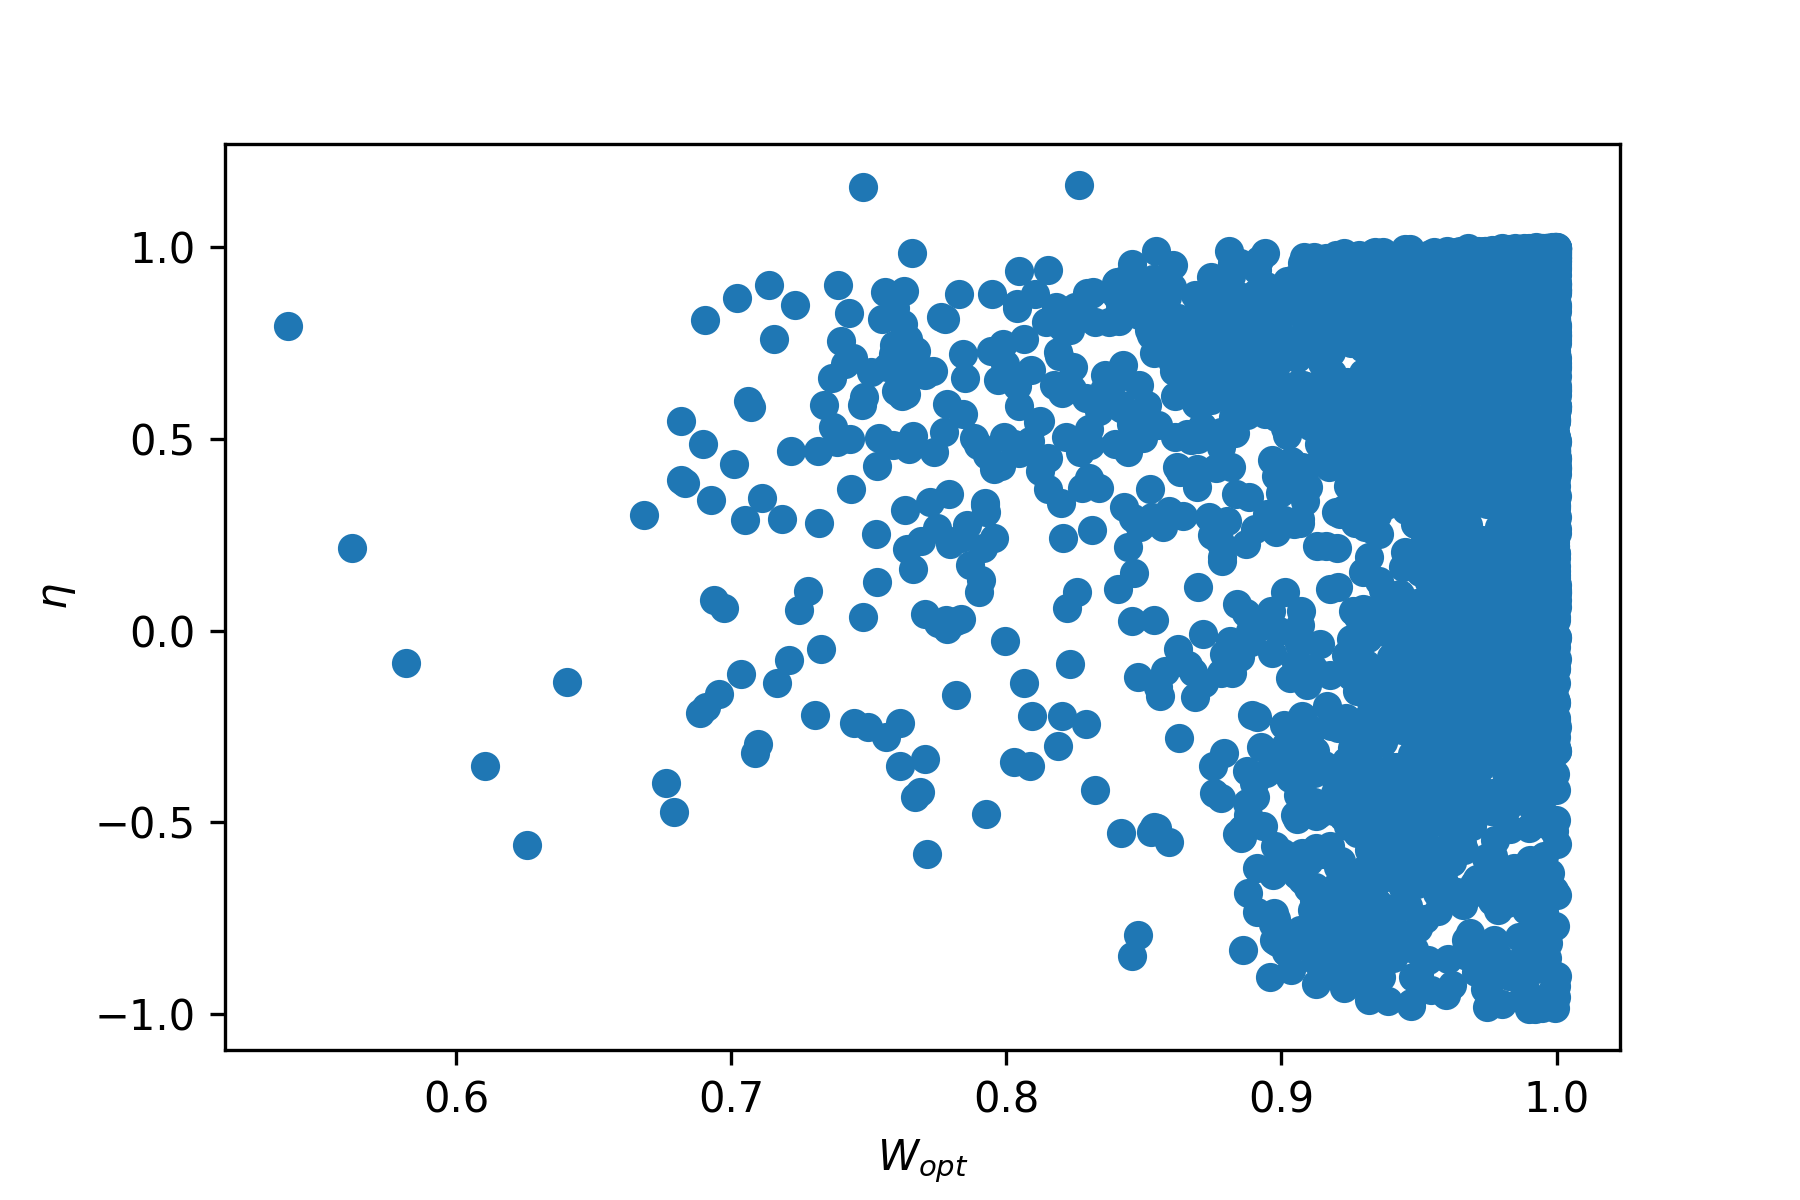
\includegraphics[width=\textwidth]{img/work_dist_n2_haar}
%		\caption{Random $\rho_0$}
%		\label{}
%	\end{subfigure}
%	\caption{}
%	\label{}
%\end{figure}
%
%
%\begin{figure}
%	\centering
%	\begin{subfigure}{0.4\textwidth}
%		\centering
%		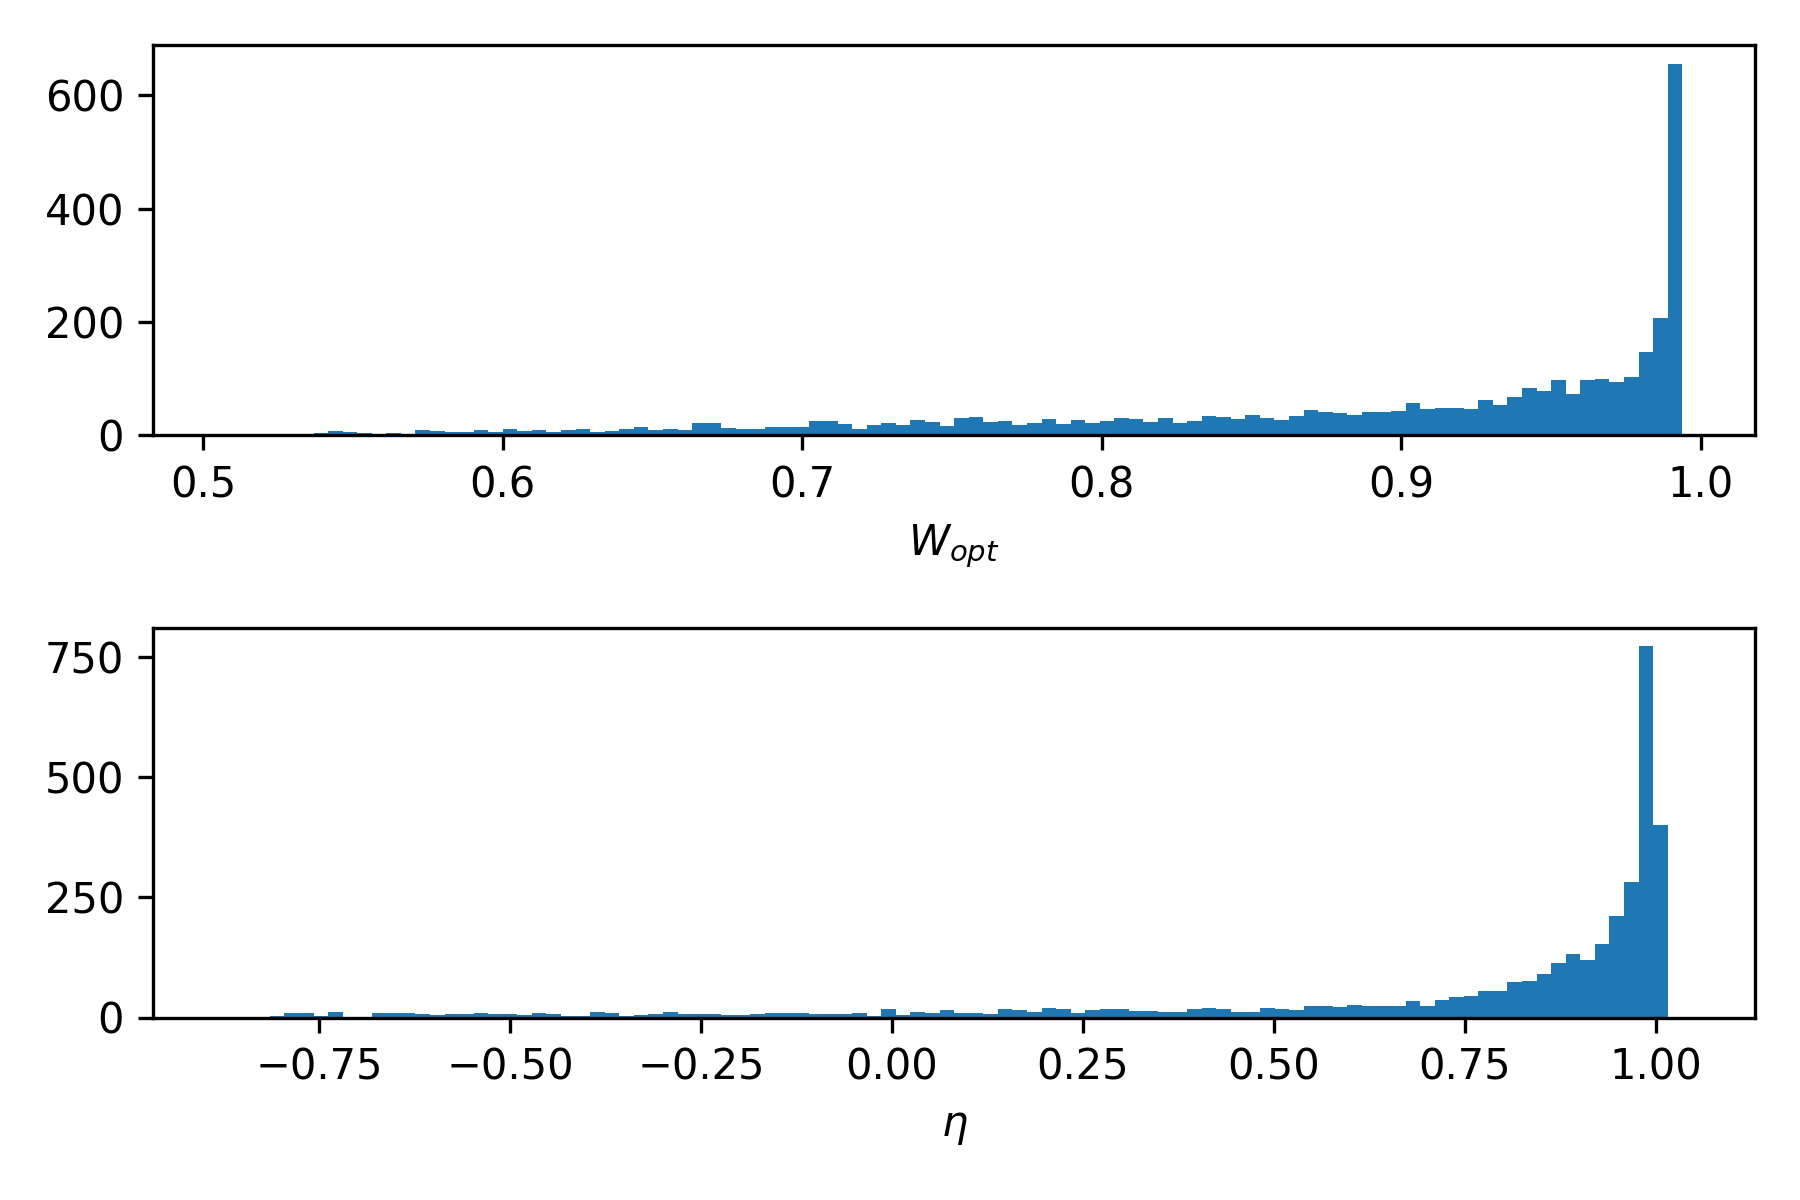
\includegraphics[width=\textwidth]{img/hist_n2_0}
%		\caption{$\rho_0 = \ket{0}\bra{0}$}
%		\label{}
%	\end{subfigure}
%	\begin{subfigure}{0.4\textwidth}
%		\centering
%		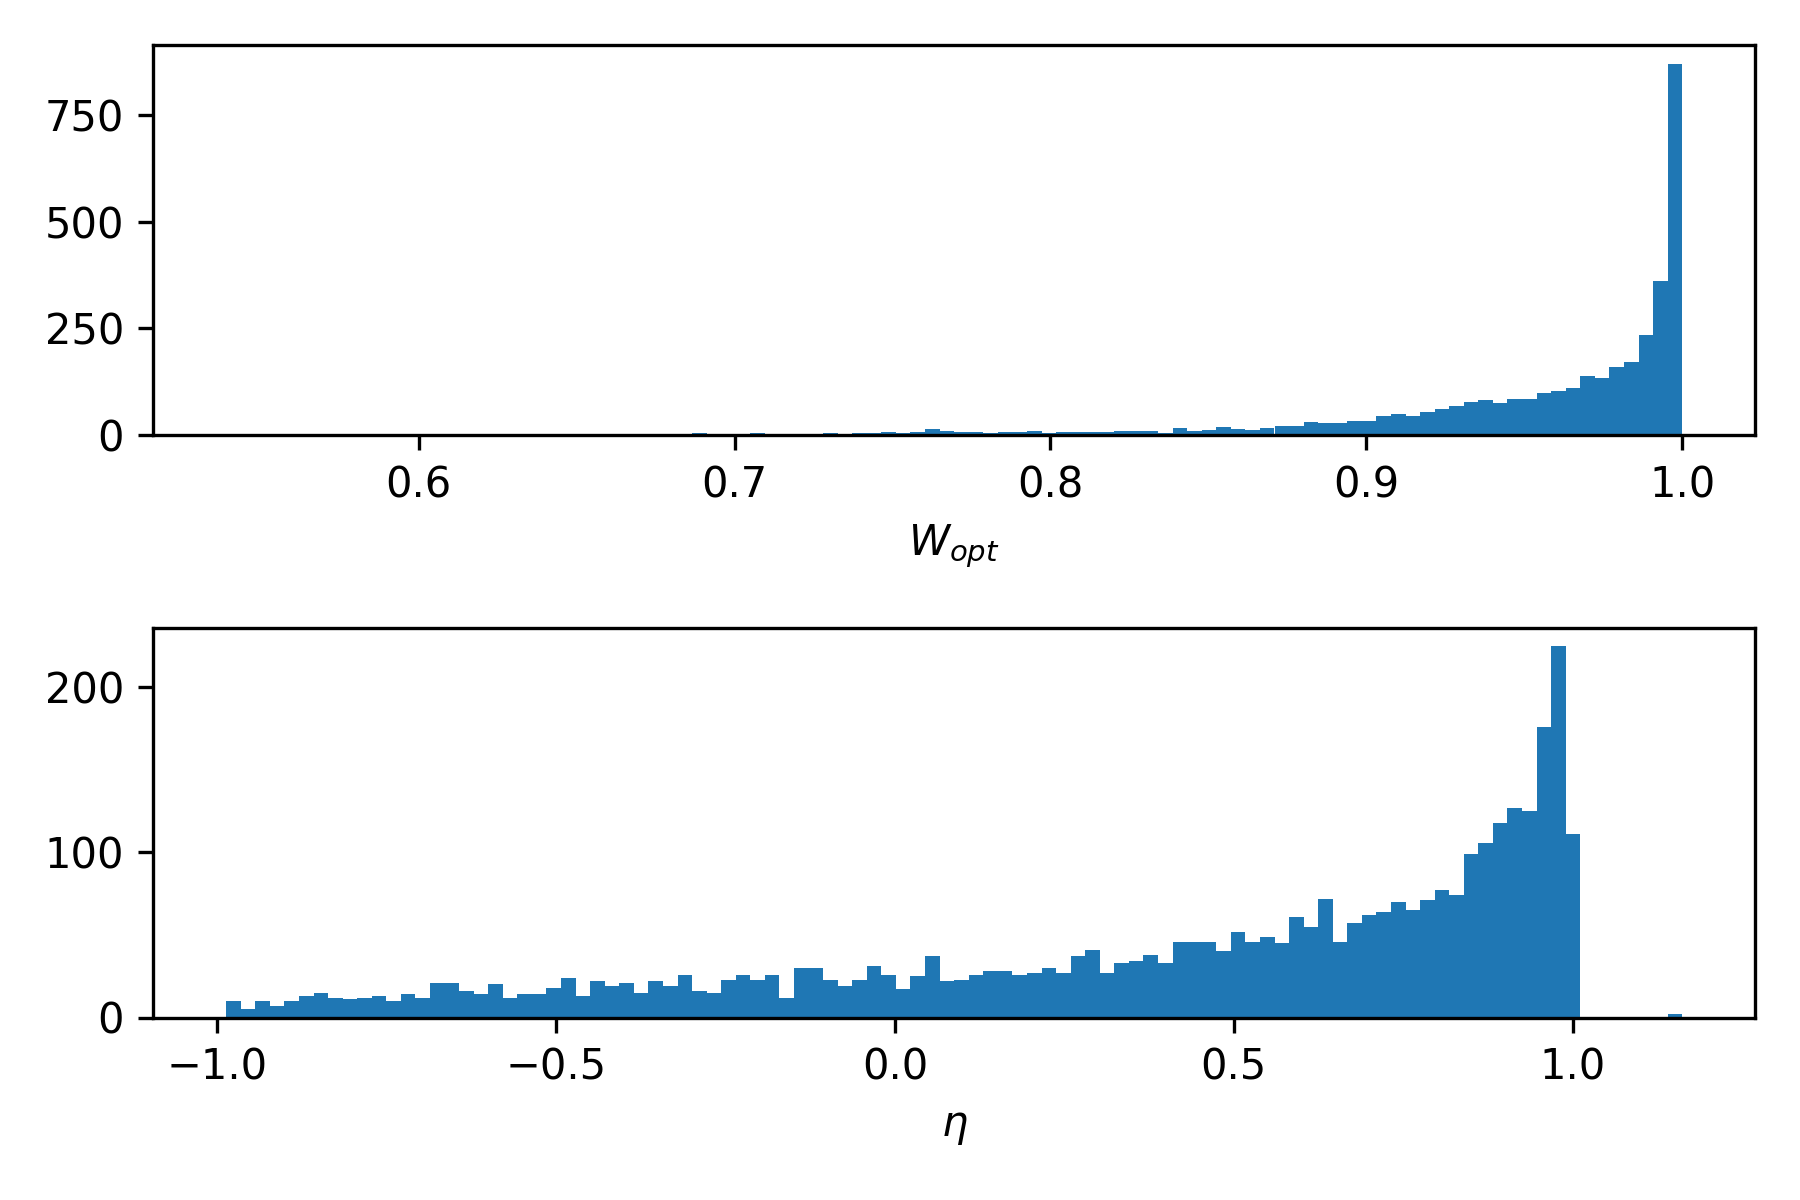
\includegraphics[width=\textwidth]{img/hist_n2_haar}
%		\caption{Random $\rho_0$}
%		\label{}
%	\end{subfigure}
%	\caption{}
%	\label{}
%\end{figure}